%% Reliable Federated TinyML Deployment for IoT Security
%% ACM SIGPLAN format (LCTES full paper: 10 pages + up to 2 pages of references and appendix).
%% Submission build: [sigplan,10pt,review,anonymous,nonacm]. Camera-ready: drop review,anonymous,nonacm
%% and add the \acmConference / copyright block supplied by the publisher.
\documentclass[sigplan,10pt,review,anonymous,nonacm]{acmart}
\settopmatter{printfolios=true,printccs=false,printacmref=false}

\usepackage{multirow}
\usepackage{adjustbox}
\usepackage{placeins}
\usepackage{xspace}
\newcommand{\cic}{CIC-IDS2017\xspace}
\newcommand{\ton}{TON\_IoT\xspace}
\newcommand{\src}[1]{\emph{Source: #1.}}
\setlength{\emergencystretch}{2em}

\begin{document}

\title{Reliable Federated TinyML Deployment for IoT Security}
\shorttitle{Reliable Federated TinyML for IoT Security}

\author{Younsoo Park}
\affiliation{\institution{Pennsylvania State University}\country{USA}}
\author{Seokhyeon Bae}
\affiliation{\institution{Pennsylvania State University}\country{USA}}

\begin{abstract}
Federated learning (FL) and TinyML together promise privacy-preserving intrusion detection on
microcontrollers, but whether a federated model can be compressed for such devices without pooled
data, and without losing detection quality, is rarely tested end to end. We train an MLP intrusion
detector with Flower on \cic and \ton and compress it for TensorFlow Lite Micro using only data that
participating clients hold. Federated training comes within 1.7 F1 points of an identically
configured centralized baseline and loses less than one F1 point under a Dirichlet(0.3) partition;
a local-only baseline shows that federation matters most for clients with few local attacks, which
detect 45--93\% of attacks alone and 99.8--99.99\% with the federated model. Structured pruning
followed by fine-tuning and QAT fine-tuning on one client's data yields a 65\,KB INT8 model
(12.3$\times$) that matches the float federated model. For recall-priority deployment, distillation
from the federated model, fine-tuning on clipped inputs across clients, and a threshold chosen on
client-held data let a 65\,KB model miss 27 of 85,173 \cic test attacks (FP32 model at its default
threshold: 52) at an 11.3\% false-alarm rate, and a 57\,KB \ton model miss 12 of 16,215 at 6.6\%.
We also find that training-time QAT inside FL collapses on heavy-tailed \cic features, that
full-integer post-training quantization is unstable across calibration draws until the calibration
inputs are clipped, and that four silent failures in a common TensorFlow/tfmot/Flower toolchain
make wrong compressed-model results look plausible; we give the checks that catch them.
\end{abstract}

\keywords{federated learning, TinyML, intrusion detection, quantization, pruning, microcontrollers}

\maketitle

%% =====================================================================
\section{Introduction}
The number of Internet of Things (IoT) devices in homes, healthcare and industrial control keeps
growing, and so does their exposure to network intrusions~\cite{atzori2010iot}. Machine-learning
intrusion detection systems (IDS) detect such traffic well~\cite{sharafaldin2018toward}, but they
are usually trained centrally on pooled traffic, which raises privacy and ownership concerns.
Federated learning (FL) lets clients train locally and share only model
updates~\cite{mcmahan2017communication,konecny2016federated}, and TinyML compresses models until
they run on microcontrollers~\cite{banbury2020benchmarking,david2021tflm}. Combining the two raises
a question that is easy to state and, as we found, easy to get wrong: can a model trained without
pooling data be compressed to microcontroller size without losing what federated training learned,
and without quietly using pooled data during compression?

Intrusion detection is a demanding test case. A missed attack usually costs more than a false
alarm, benchmark datasets are imbalanced, and their standardized features are heavy-tailed. We
study this combination on two datasets with an MLP detector and make five contributions:
\begin{itemize}
\item An end-to-end evaluation of federated training against an identically configured centralized
  baseline under near-IID and Dirichlet(0.3) partitions, together with a local-only baseline that
  locates the benefit of federation in clients with few local attacks (\S\ref{sec:fl}).
\item An FL-faithful compression procedure (exact BatchNorm folding, structured pruning, fine-tuning
  and QAT fine-tuning on one client's data) and its decomposition, compression-strength sweep, and
  dependence on the fine-tuning client (\S\ref{sec:compression}).
\item A comparison of five post-training quantization methods and 16 complete pipelines combining
  structured and unstructured pruning, PTQ, QAT and distillation, including the instability of
  full-integer PTQ across calibration draws and a one-line fix (\S\ref{sec:quant},\S\ref{sec:combos}),
  and a comparison with calibration estimators, PTQ-initialized and learned-clipping QAT, and
  server-side data-free calibration from the literature, which locates the problem in the input
  quantization range (\S\ref{sec:quantlit}).
\item A recall-priority deployment recipe that uses only client-held data and lets compressed
  models miss fewer attacks than the FP32 model at its default threshold (\S\ref{sec:recall}).
\item A negative result for training-time QAT inside FL on heavy-tailed features, and four silent
  toolchain failure modes with the invariant check that exposes them (\S\ref{sec:qatfl},\S\ref{sec:failures}).
\end{itemize}
The paper is an evidence-backed characterization rather than a new algorithm. All numbers come from
our own runs; the table captions name the run that produced them (Appendix~\ref{app:provenance}).

%% =====================================================================
\section{Background and Related Work}
\paragraph{Intrusion detection datasets.} \cic~\cite{sharafaldin2018toward} is the most widely used
flow-based IDS benchmark; Engelen et al.~\cite{engelen2021troubleshooting} document labelling and
flow-construction errors in it, which makes absolute numbers hard to compare across papers.
\ton~\cite{moustafa2021toniot} and Bot-IoT~\cite{koroniotis2019botiot} target IoT traffic. We use
\cic and the \ton network dataset.

\paragraph{Federated learning.} FedAvg~\cite{mcmahan2017communication} averages client updates;
FedAvgM~\cite{hsu2019measuring}, which we use, adds server momentum and is evaluated there on
Dirichlet label partitions, the non-IID model we adopt. Zhao et al.~\cite{zhao2018federated}
characterize the degradation under skewed client data, and FedProx~\cite{li2020fedprox} adds a
proximal term for the same reason. We use the Flower framework~\cite{beutel2020flower}.

\paragraph{TinyML and compression.} TensorFlow Lite Micro (TFLM)~\cite{david2021tflm} runs integer
and float models on microcontrollers~\cite{banbury2020benchmarking}. Pruning~\cite{han2016deep},
distillation~\cite{hinton2015distilling} and quantization~\cite{jacob2018quantization} reduce model
size; surveys and guidance on PTQ and QAT are given by Gholami et al.~\cite{gholami2021survey} and
Nagel et al.~\cite{nagel2021white}, who also describe oscillation-driven QAT
instability~\cite{nagel2022overcoming}. Section~\ref{sec:qatfl} reports a different, data-driven QAT
failure.

\paragraph{Calibration and quantization ranges.} Post-training calibration can clip activation ranges
instead of using their extremes: percentile and entropy (KL) calibration~\cite{wu2020integer}, or the
MSE-optimal clip of ACIQ~\cite{banner2019aciq}. Wu et al.\ also recommend calibrating first and then
fine-tuning with QAT~\cite{wu2020integer}. PACT~\cite{choi2018pact} and LSQ~\cite{esser2020lsq} learn
the clip or step size during QAT, and DFQ~\cite{nagel2019dfq} quantizes without data by equalizing
weight ranges across layers (CLE). Distillation and quantization have been combined
before~\cite{polino2018model}, and tfmot provides sparsity-preserving QAT because standard QAT
re-densifies pruned weights~\cite{tfmot2021collab}. In FL, quantization has mainly been used to
compress updates~\cite{reisizadeh2020fedpaq}; Gupta et al.\ train federated models that stay accurate
under later quantization~\cite{gupta2023quantization}. Our input clipping is an instance of clipped
calibration; Section~\ref{sec:quantlit} compares it with these estimators and with QAT-range,
data-free and learned-clipping variants on our models.

\paragraph{Robustness of compressed models.} FGSM~\cite{goodfellow2015fgsm} and
PGD~\cite{madry2018towards} are the standard gradient attacks. Quantization can improve or degrade
robustness depending on attack strength~\cite{gorsline2021adversarial}; weight
quantization~\cite{song2021improving} and deep quantization~\cite{ayaz2023improving} interact with
adversarial training. We measure whether the federated model's robustness carries over to its INT8
derivatives.

%% =====================================================================
\section{Method}\label{sec:method}
\subsection{Datasets and Preprocessing}\label{sec:data}
\paragraph{\cic~\cite{sharafaldin2018toward}.} The eight MachineLearningCSV files (2,830,743 flows,
78 numeric features). Labels are binarized (benign vs.\ any attack), $\pm\infty$ and non-numeric
values are replaced, and duplicate rows are removed before any split (2,499,543 unique flows, 425,863
attacks). A stratified 80/20 split gives a test set of 499,909 flows (85,173 attacks) at the natural
class ratio. On the training split only, the majority class is undersampled to at most 4:1, a
StandardScaler is fitted, and SMOTE~\cite{chawla2002smote} balances the classes.

\paragraph{\ton~\cite{moustafa2021toniot}.} The network train/test file (211,043 records). We drop
host identifiers and ephemeral ports (src\_ip, dst\_ip, src\_port) to avoid shortcut features and
keep dst\_port. Text columns with at most 50 distinct values are label-encoded. The high-cardinality
DNS query and URI fields are not used directly; instead we add six row-local features (length, digit
count and non-alphanumeric count of each field), which cannot leak information across records, for
43 features. Deduplication on the other 37 features leaves 105,176 records (81,070 attacks); the
test set has 21,036 records (16,215 attacks). The same balancing, scaling and SMOTE steps follow. The
text-derived features and the \ton focal-loss setting were selected on validation data
(Appendix~\ref{app:tonrecipe}).

\subsection{Federated Training}\label{sec:fltrain}
The model is an MLP (512--256--128, ReLU, each hidden layer followed by BatchNorm and Dropout,
sigmoid output). We train it with Flower~\cite{beutel2020flower} on four clients with FedAvgM (server
momentum 0.5, server learning rate 0.1)~\cite{hsu2019measuring}, 60 rounds $\times$ 3 local epochs,
batch size 128, Adam, and a server-broadcast cosine learning-rate schedule
($10^{-3}\rightarrow10^{-4}$). Class imbalance is handled with focal loss~\cite{lin2017focal}
($\alpha=0.35$ for \cic; $\alpha=0.5$ for \ton, where attacks are the majority) and class weights.
Clients receive either a near-IID partition (each class split evenly) or a Dirichlet($\alpha=0.3$)
label partition~\cite{hsu2019measuring}. The centralized baseline trains the identical model and loss
for the same 180 epochs.

\subsection{FL-Faithful Compression}\label{sec:fcomp}
After training, the server holds only the global float model. (1) BatchNorm is folded exactly.
Because it follows the ReLU, it is folded into the \emph{next} Dense layer
(Appendix~\ref{app:bn}; maximum deviation $\le2\cdot10^{-5}$). (2) Structured pruning removes 50\% of
the neurons of each hidden layer by weight magnitude. (3) One participating client fine-tunes the
pruned model for 3 epochs on 10,000 of its own samples. (4) The same client performs 2 epochs of QAT
fine-tuning~\cite{jacob2018quantization}, and the model is exported as INT8 TFLite. We call this the
\emph{base recipe}. Fine-tuning on 10,000 pooled samples is reported only as an upper bound, because
a federated server would not hold them.

\subsection{Recall-Priority Deployment}\label{sec:recallmethod}
For deployments that must miss as few attacks as possible we extend the base recipe in three ways
that use only client-held data: (a) fine-tuning targets $0.5\,y + 0.5\,\sigma(z_{\text{teacher}}/2)$,
i.e.\ distillation~\cite{hinton2015distilling} from the federated model at temperature 2; (b) inputs
clipped to $\pm5$ standard deviations during fine-tuning and calibration; (c) optionally, federated
fine-tuning, in which all clients fine-tune and the server averages the weights after every epoch.
The decision threshold is the largest value that reaches a target attack recall on a held-out part
of the fine-tuning client's data (20,000 samples for \cic, 8,000 for \ton), disjoint from every
fine-tuning draw. The test split is never used for selection.

\subsection{Evaluation}\label{sec:eval}
Unless stated otherwise, metrics are computed on the test split at a fixed threshold of 0.3, chosen
before these experiments. We report accuracy, precision, attack recall, F1, the false-alarm rate (FAR,
the share of benign records flagged), and the number of missed attacks out of all test attacks.
Robustness uses FGSM and PGD ($\epsilon=0.1$ on standardized features; PGD with 10 steps); adversarial
examples are computed on the float federated model and transferred to all other models. Where
fine-tuning or calibration involves random draws, we repeat it three to five times and report the
mean and range.

\paragraph{Setup.} All runs used one desktop (16-core CPU under WSL2; Flower simulates the clients
on CPU). A \cic federated run takes about 5.4\,h, a \ton run about 25\,min. Code, configurations,
logs and per-run result files are in the artifact repository; Appendix~\ref{app:provenance} maps every
table to its run.

%% =====================================================================
\section{Results}
\subsection{Federated Training and Where Federation Helps}\label{sec:fl}

\begin{table*}[t]
\caption{Federated vs.\ centralized training and the effect of a Dirichlet(0.3) partition (float
models, test split, threshold 0.3). \src{\cic runs B, I; \ton runs S, U}}
\label{tab:fl}
\small
\begin{adjustbox}{max width=\textwidth}
\begin{tabular}{llrrrrrr}
\toprule
Dataset & Model & Accuracy & Precision & Attack recall & F1 & FAR & Missed / all attacks \\
\midrule
\multirow{4}{*}{\cic} & Centralized & 95.07\% & 77.60\% & 99.90\% & 87.35 & 5.92\% & 88 / 85,173 (0.10\%) \\
 & Federated, near-IID & 94.32\% & 75.01\% & 99.94\% & 85.70 & 6.84\% & 52 / 85,173 (0.061\%) \\
 & Federated, fixed learning rate & 95.01\% & 77.40\% & 99.84\% & 87.20 & 5.99\% & 136 / 85,173 (0.16\%) \\
 & Federated, Dirichlet(0.3) & 94.27\% & 74.91\% & 99.83\% & 85.59 & 6.87\% & 144 / 85,173 (0.17\%) \\
\midrule
\multirow{5}{*}{\ton} & Centralized & 99.51\% & 99.43\% & 99.94\% & 99.68 & 1.93\% & 10 / 16,215 (0.062\%) \\
 & Federated, near-IID & 99.08\% & 98.94\% & 99.88\% & 99.41 & 3.61\% & 19 / 16,215 (0.12\%) \\
 & Federated, second training run & 99.04\% & 98.91\% & 99.86\% & 99.38 & 3.71\% & 23 / 16,215 (0.14\%) \\
 & Federated, fixed learning rate & 98.97\% & 98.82\% & 99.86\% & 99.34 & 4.00\% & 23 / 16,215 (0.14\%) \\
 & Federated, Dirichlet(0.3) & 97.81\% & 97.25\% & 99.99\% & 98.60 & 9.52\% & 1 / 16,215 (0.006\%) \\
\bottomrule
\end{tabular}
\end{adjustbox}
\end{table*}

Federated training comes within 1.65 F1 points of centralized training on \cic and within 0.27 on
\ton (Table~\ref{tab:fl}); on both datasets the gap lies mostly in precision, and all models detect
more than 99.8\% of attacks. A second, independent \ton training run differs by 0.03 F1. A fixed
learning rate does as well as the cosine schedule (F1 87.20 vs.\ 85.70 and 99.34 vs.\ 99.41), so we
do not claim a benefit for the schedule. The Dirichlet partition is extreme: on \cic one client holds
73\% of the training data and two clients see almost no attacks. Federated training still loses only
0.11 F1 on \cic and 0.81 on \ton, where the model becomes recall-heavy (one missed attack, FAR 9.5\%).

\begin{table}[t]
\caption{Each client trained alone (10 epochs, $\le$200k samples) vs.\ the federated model of the
same partition; recall and missed attacks on the test split. \src{runs K, V; federated rows as
Table~\ref{tab:fl}}}
\label{tab:local}
\small
\setlength{\tabcolsep}{3.5pt}
\begin{adjustbox}{max width=\columnwidth}
\begin{tabular}{lrrr}
\toprule
Client (attack share) & Recall alone & Missed alone & Federated \\
\midrule
\cic near-IID, each (50\%) & 98.85--99.78\% & 185--982 & 52 \\
\cic Dir.\ client 0 (0.1\%) & 44.97\% & 46,872 & \multirow{2}{*}{144} \\
\cic Dir.\ client 2 (2.6\%) & 91.11\% & 7,572 & \\
\ton near-IID, each (50\%) & 99.69--99.81\% & 31--51 & 19 \\
\ton Dir.\ client 0 (0.4\%) & 85.53\% & 2,346 & \multirow{2}{*}{1} \\
\ton Dir.\ client 3 (8.5\%) & 93.39\% & 1,072 & \\
\bottomrule
\end{tabular}
\end{adjustbox}
\end{table}

Table~\ref{tab:local} shows where federation pays off. Clients whose local data contains few attacks
detect only 45--93\% of attacks when trained alone; on the same partitions the federated model
detects 99.83\% (\cic) and 99.99\% (\ton). Clients that already hold large, representative data gain
little: on near-IID \cic each client alone reaches F1 88.3--90.0 (federated: 85.70) at a
precision-heavier operating point that misses 3.6--19 times as many attacks. The near-IID partition is
therefore the setting in which federation is least needed. Local and federated training budgets are
not matched, and at a fixed threshold the F1 differences among data-rich clients mainly reflect
operating points.

%% ---------------------------------------------------------------------
\subsection{Compression Without Pooled Data}\label{sec:compression}

\begin{table*}[t]
\caption{Compression of the near-IID federated model. ``Client FT'' uses 10,000 samples of client
0's own data; ``pooled'' uses 10,000 pooled samples a federated server would not hold. The rows
without fine-tuning calibrate INT8 on 500 pooled samples (one draw; see \S\ref{sec:quant}).
\src{\cic run E; \ton run V}}
\label{tab:compression}
\small
\begin{adjustbox}{max width=\textwidth}
\begin{tabular}{lrrrrrr}
\toprule
 & \multicolumn{3}{c}{\cic} & \multicolumn{3}{c}{\ton} \\
\cmidrule(lr){2-4}\cmidrule(lr){5-7}
Variant & Size & F1 / FAR & Missed of 85,173 & Size & F1 / FAR & Missed of 16,215 \\
\midrule
FP32 federated model (TFLite) & 802.5\,KB & 85.70 / 6.84\% & 52 & 732.4\,KB & 99.41 / 3.61\% & 19 \\
INT8 PTQ only & 226.9\,KB & 84.75 / 7.37\% & 74 & 209.4\,KB & 98.96 / 3.86\% & 153 \\
Prune 50\%, no fine-tuning $\rightarrow$ PTQ & 75.1\,KB & 42.28 / 56.04\% & 46 & 66.3\,KB & 95.30 / 30.20\% & 129 \\
Prune 50\% $\rightarrow$ client FT $\rightarrow$ PTQ & 75.1\,KB & 86.90 / 6.08\% & 346 & 66.3\,KB & 90.20 / 13.23\% & 2,369 \\
Prune 50\% $\rightarrow$ client FT $\rightarrow$ QAT FT (base recipe) & 65.4\,KB & 85.59 / 6.82\% & 291 & 56.7\,KB & 98.67 / 2.26\% & 319 \\
Same, pooled fine-tuning (upper bound) & 65.4\,KB & 90.72 / 2.98\% & 4,216 & 56.7\,KB & 99.16 / 3.48\% & 105 \\
\bottomrule
\end{tabular}
\end{adjustbox}
\end{table*}

INT8 PTQ alone gives 3.5$\times$ at a cost of about one F1 point for the calibration draw used in
Table~\ref{tab:compression}, but that cost varies widely between draws (\S\ref{sec:quant}). Pruning
half of each hidden layer gives a further 3.5$\times$ only if the pruned model is fine-tuned; without
fine-tuning it breaks down (F1 42.28 on \cic, FAR 30\% on \ton). With fine-tuning and QAT fine-tuning
on one client's data, the INT8 model is 65.4\,KB on \cic (12.27$\times$) and 56.7\,KB on \ton
(12.92$\times$) and stays close to the float model (F1 85.59 vs.\ 85.70 and 98.67 vs.\ 99.41). The QAT
fine-tuning step matters: client-fine-tuned PTQ reaches only F1 90.20 on \ton. Pooled fine-tuning
scores a higher \cic F1 only by moving toward precision; it misses 4,216 attacks instead of 291.

\paragraph{Which client fine-tunes.} The fine-tuning client's class mix shifts the operating point.
On the \cic Dirichlet model, fine-tuning on client 3 (24.9\% attacks) gives the highest F1 we
observed (91.08, FAR 2.75\%) but misses 4,415 attacks, fifteen times as many as the near-IID model
fine-tuned on a 50\%-attack client. On \ton, client 2 of the Dirichlet run gives F1 98.80 (248 missed).
\src{runs E, V}

\paragraph{Compression strength.} Figure~\ref{fig:sweep} sweeps the pruning ratio from 30\% to 90\%.
Without fine-tuning, pruning collapses from 50\% (\cic) or 85\% (\ton) onward. With client fine-tuning,
\cic degrades gracefully (70\%: 31\,KB, F1 84.4--85.0; 90\%: 9.9\,KB, F1 78.0), and on \ton client
fine-tuning + QAT holds F1 98.65--98.74 down to 8.2\,KB (90$\times$ smaller than FP32), whereas client
fine-tuning + PTQ stays at 87.7--91.5. QAT fine-tuning is the choice that is reliable on both datasets.

\begin{figure*}[t]
\centering
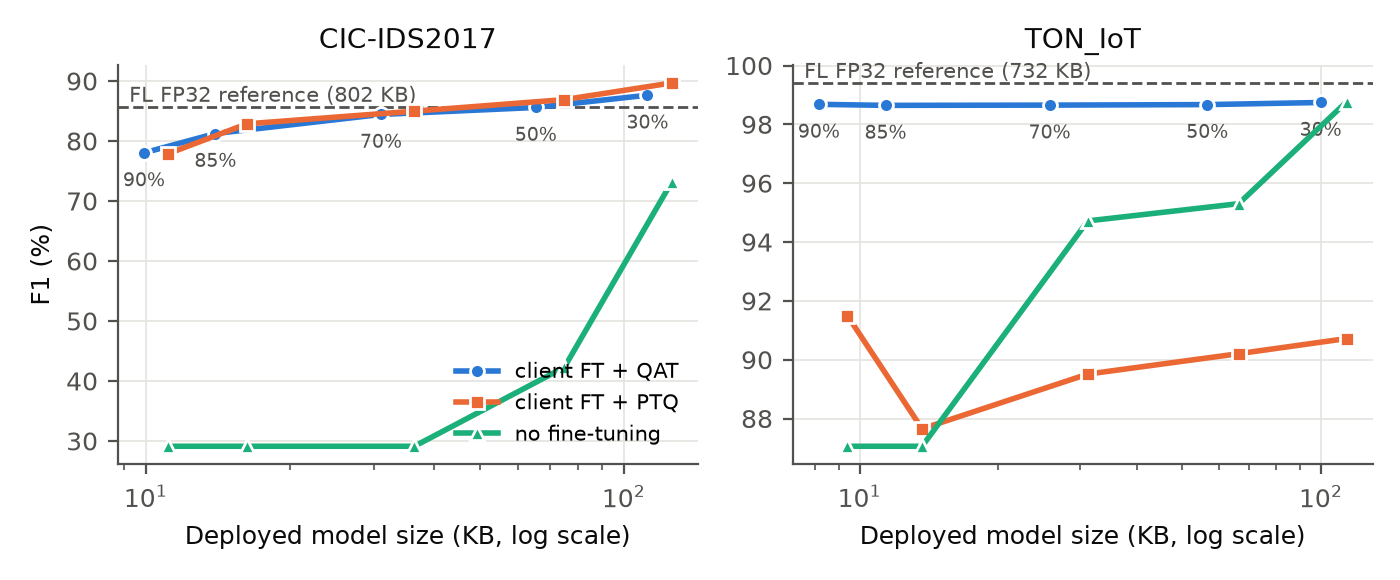
\includegraphics[width=0.82\textwidth]{figures/prune_sweep.png}
\caption{F1 vs.\ deployed INT8 size for structured pruning ratios 30--90\% (labels), with client
fine-tuning followed by QAT fine-tuning or PTQ, and without fine-tuning. Dashed: uncompressed
federated model. \src{\cic run G; \ton run W}}
\Description{Two line charts of F1 against model size on a log scale. For CIC-IDS2017, the
fine-tuned curves fall from about 89 at 126 KB to 78 at 10 KB while the no-fine-tuning curve collapses
below 50 KB. For TON_IoT, the QAT curve stays near 98.7 from 100 KB to 8 KB, the PTQ curve stays near
88 to 91, and the no-fine-tuning curve falls to 87.}
\label{fig:sweep}
\end{figure*}

%% ---------------------------------------------------------------------
\subsection{Quantization Methods and Calibration}\label{sec:quant}

\begin{table*}[t]
\caption{Post-training quantization methods: size and F1 (calibration: one draw of 500 client-0
samples). ``Pruned'' = prune 50\% $\rightarrow$ client FT. TFLM = runs on the TFLM build we deploy.
\src{\cic run J; \ton run V}}
\label{tab:quantmethods}
\small
\begin{adjustbox}{max width=\textwidth}
\begin{tabular}{lcrrrrrrrr}
\toprule
 & & \multicolumn{4}{c}{\cic} & \multicolumn{4}{c}{\ton} \\
\cmidrule(lr){3-6}\cmidrule(lr){7-10}
 & & \multicolumn{2}{c}{Federated} & \multicolumn{2}{c}{Pruned + client FT} & \multicolumn{2}{c}{Federated} & \multicolumn{2}{c}{Pruned + client FT} \\
Method & TFLM & Size & F1 & Size & F1 & Size & F1 & Size & F1 \\
\midrule
FP32 & yes & 802\,KB & 85.70 & 243\,KB & 89.39 & 732\,KB & 99.41 & 208\,KB & 99.42 \\
Dynamic range (INT8 weights, float compute) & no & 216\,KB & 85.58 & 69\,KB & 90.13 & 199\,KB & 99.41 & 61\,KB & 99.43 \\
Float16 weights & no & 404\,KB & 85.70 & 124\,KB & 89.35 & 369\,KB & 99.41 & 106\,KB & 99.42 \\
Full-integer INT8 & yes & 227\,KB & 85.02 & 75\,KB & 86.90 & 209\,KB & 97.69 & 66\,KB & 90.20 \\
int16x8 (INT8 weights, 16-bit activations) & untested & 238\,KB & 85.48 & 81\,KB & 89.61 & 220\,KB & 99.40 & 72\,KB & 99.41 \\
\bottomrule
\end{tabular}
\end{adjustbox}
\end{table*}

Every method that keeps activations in float or 16 bits loses at most 0.25 F1
(Table~\ref{tab:quantmethods}). Full-integer INT8 is the only lossy method (\ton pruned model: 9.2 F1,
FAR 2.0\%$\rightarrow$13.2\%); since int16x8 uses the same INT8 weights and recovers, the loss comes
from 8-bit activations. The TFLM build we deploy runs only FP32 and full-integer INT8 kernels, so
dynamic range (the best size--accuracy point on \cic) suits Linux-class gateways but not the
microcontroller.

\begin{table}[t]
\caption{Full-integer PTQ of the federated models over 15 calibration sets per size (5 sources
$\times$ 3 random draws): median F1, minimum F1, and sets within 1 F1 of FP32. \src{\cic runs L, M;
\ton run V}}
\label{tab:calib}
\small
\setlength{\tabcolsep}{3pt}
\begin{adjustbox}{max width=\columnwidth}
\begin{tabular}{lrrrrrr}
\toprule
 & \multicolumn{3}{c}{\ton (FP32 99.41)} & \multicolumn{3}{c}{\cic (FP32 85.70)} \\
\cmidrule(lr){2-4}\cmidrule(lr){5-7}
Calibration & Med. & Min. & $\le$1 & Med. & Min. & $\le$1 \\
\midrule
100 samples & 99.36 & 96.11 & 14/15 & 84.60 & 81.47 & 5/15 \\
500 samples & 99.37 & 54.01 & 13/15 & 83.11 & 80.91 & 2/15 \\
2,000 samples & 97.68 & 32.72 & 5/15 & 82.60 & 29.16 & 1/15 \\
2,000, clipped $\pm5$ & 99.19 & 99.19 & 15/15 & 84.61 & 83.02 & 4/15 \\
\bottomrule
\end{tabular}
\end{adjustbox}
\end{table}

Full-integer PTQ is also unstable (Table~\ref{tab:calib}). The calibration source (pooled data or any
client) does not matter, but the random draw does: the same \ton model ranges from F1 32.7 to 99.4 and
the \cic model from 29.2 to 85.0, and more calibration data makes it worse. The TFLite converter sets
each activation range from the minimum and maximum it sees, and a larger calibration set is more
likely to contain an extreme record of the heavy-tailed standardized features: the worst conversions
have hidden-layer maxima near 400 (\ton) and 9,609 (\cic), against roughly 50--210 for most others. A
one-line change removes the instability: clipping calibration inputs to $\pm5$ standard deviations
gives F1 99.19 for every \ton set and 83.0--84.9 on \cic ($\pm10$ works as well; $\pm3$ is too tight).
QAT fine-tuning is more stable, though not draw-independent (\S\ref{sec:quantlit} explains why):
over five fine-tuning draws the base recipe gives F1 98.79--99.51 on \ton (PTQ: 96.89--99.19) and
86.77--89.28 on \cic (PTQ: 79.37--89.05). Table~\ref{tab:compression}'s \cic value (85.59) lies below
all five draws, so it is conservative rather than selected.

\subsection{Calibration Estimators, QAT Ranges and Data-Free Calibration}\label{sec:quantlit}
We tested the methods of Section~2 on the federated models (Tables~\ref{tab:qlit-ptq}
and~\ref{tab:qlit-qat}). To compare range estimators with everything else fixed, we build the tfmot
fake-quantization model, set its activation ranges directly and convert it; with min/max ranges this
reproduces TFLite's per-tensor PTQ exactly (same F1, FAR and misses on every set). TFLite's default
PTQ uses per-channel weight scales, QAT exports use per-tensor scales.

\begin{table*}[t]
\caption{Full-integer PTQ of the unpruned federated models with different range estimators: F1 mean
[minimum], missed attacks (mean), FAR (mean). Real-data rows: the 15 calibration sets of
Table~\ref{tab:calib} (2,000 samples). Data-free rows use no client data (synthetic: 3 draws of 2,000
$\mathcal{N}(0,I)$ inputs; BN: ranges $\mu+k\sigma$ from the federated BatchNorm statistics). CLE =
cross-layer equalization~\cite{nagel2019dfq}. \src{runs X1, X3}}
\label{tab:qlit-ptq}
\small
\begin{adjustbox}{max width=\textwidth}
\begin{tabular}{llrrrrrr}
\toprule
 & & \multicolumn{3}{c}{\cic (85,173 attacks)} & \multicolumn{3}{c}{\ton (16,215 attacks)} \\
\cmidrule(lr){3-5}\cmidrule(lr){6-8}
Weights & Range estimator & F1 [min] & Missed & FAR & F1 [min] & Missed & FAR \\
\midrule
per-channel & min/max (TFLite default) & 77.67 [29.16] & 349 & 15.51 & 77.91 [32.72] & 4,779 & 2.99 \\
per-channel & inputs clipped $\pm$5 SD (ours) & 84.38 [83.02] & 68 & 7.58 & 99.19 [99.19] & 27 & 4.94 \\
per-tensor & min/max & 76.64 [29.20] & 397 & 16.14 & 81.00 [36.06] & 4,156 & 4.48 \\
per-tensor & percentile 99.9~\cite{wu2020integer} & 83.16 [82.11] & 58 & 8.30 & \textbf{99.39 [99.38]} & 26 & 3.55 \\
per-tensor & percentile 99.99 & 79.27 [31.51] & 543 & 13.34 & 99.31 [98.81] & 50 & 3.62 \\
per-tensor & MSE-optimal clip (ACIQ objective~\cite{banner2019aciq}) & 77.28 [29.28] & 630 & 15.50 & 88.68 [34.62] & 2,395 & 4.72 \\
per-tensor & KL / entropy~\cite{wu2020integer} & 80.93 [44.16] & 565 & 10.68 & 98.97 [96.69] & 131 & 4.20 \\
per-tensor & inputs clipped $\pm$5 SD & 82.93 [82.09] & 239 & 8.37 & 99.19 [99.18] & 27 & 4.94 \\
per-tensor & CLE + inputs clipped $\pm$5 SD (3 sets) & 84.46 [84.04] & 58 & 7.54 & 99.18 [99.18] & 29 & 4.93 \\
\midrule
per-channel & data-free: synthetic $\mathcal{N}(0,I)$ inputs & 82.22 [80.58] & 54 & 8.87 & 99.16 [99.08] & 29 & 5.06 \\
per-tensor & data-free: BN statistics, $k=4$ & 83.03 & 72 & 8.37 & 99.17 & 26 & 5.06 \\
per-tensor & data-free: BN statistics, $k=6$ & 82.51 & 66 & 8.69 & 99.26 & 27 & 4.44 \\
per-tensor & data-free: CLE + BN statistics, $k=6$ & \textbf{84.64} & 55 & 7.44 & 99.25 & 30 & 4.48 \\
\midrule
 & FP32 federated model & 85.70 & 52 & 6.84 & 99.41 & 19 & 3.61 \\
\bottomrule
\end{tabular}
\end{adjustbox}
\end{table*}

\paragraph{Estimators.} Only estimators that clip hard remove the collapses: the 99.9th percentile and
our $\pm5$\,SD input clip. The 99.99th percentile, the MSE-optimal clip and KL calibration still fail
on some calibration sets (minimum F1 29--44 on \cic, 35--97 on \ton). The rare extreme records that
stretch the ranges are too rare to move a per-tensor MSE or KL objective. With the same per-tensor
weights, the 99.9th percentile is at least as good as our clip (\ton FAR 3.55\% vs.\ 4.94\%, \cic
misses 58 vs.\ 239). Per-channel weights barely change min/max calibration, but with clipped inputs
they cut \cic misses from 239 to 68; CLE recovers the same effect for per-tensor weights (58).

\paragraph{Data-free calibration.} The server can calibrate without any client data. Because inputs
are standardized, synthetic $\mathcal{N}(0,I)$ inputs are a usable calibration set, and the federated
BatchNorm statistics (averaged by FedAvg like any weight) give each post-ReLU activation's mean and
standard deviation; we set the range to $\max_c(\mu_c+k\sigma_c)$. Both match clipped real-data
calibration on both datasets, and CLE plus BN statistics ($k=6$) gives the best \cic PTQ result
(84.64, 55 misses). $k=3$ is too tight (\cic 532, \ton 282 misses).

\begin{table}[t]
\caption{QAT ranges on the base recipe (prune 50\%, client FT, 2 QAT epochs, 5 FT draws): F1 mean
[range], missed attacks (mean). ``Start'': ranges initialized from client calibration and then updated
by tfmot (5 estimators, range of means); ``fixed'': held at the calibrated values. \src{runs X2, X4}}
\label{tab:qlit-qat}
\small
\setlength{\tabcolsep}{2pt}
\begin{adjustbox}{max width=\columnwidth}
\begin{tabular}{lrrrr}
\toprule
 & \multicolumn{2}{c}{\cic} & \multicolumn{2}{c}{\ton} \\
\cmidrule(lr){2-3}\cmidrule(lr){4-5}
Variant & F1 & Missed & F1 & Missed \\
\midrule
PTQ, min/max (TFLite) & 85.81 [79.4--89.1] & 562 & 98.62 [96.9--99.2] & 351 \\
QAT, tfmot default & 88.02 [86.8--89.3] & 513 & 99.00 [98.8--99.5] & 204 \\
QAT, calibrated start & 87.79--88.18 & 447--664 & 98.99--99.03 & 194--208 \\
QAT, fixed min/max & \textbf{89.49} [87.4--91.4] & 757 & 99.46 [99.4--99.5] & 74 \\
QAT, fixed pct.\ 99.99 & 88.58 [87.4--90.0] & \textbf{392} & \textbf{99.47} [99.4--99.5] & \textbf{70} \\
QAT, fixed MSE & 88.62 [87.3--90.1] & 839 & 99.47 [99.4--99.6] & 76 \\
QAT, fixed $\pm$5\,SD & 88.10 [87.4--89.0] & 598 & 99.34 [99.2--99.4] & 79 \\
QAT, learned clip (PACT-style) & 87.67--88.73 & 652--718 & 98.99--99.00 & 199--208 \\
\bottomrule
\end{tabular}
\end{adjustbox}
\end{table}

\paragraph{QAT ranges and order.} tfmot's default QAT does not learn its ranges in a fine-tuning run
this short. Activation ranges start at $\pm6$ and follow an exponential moving average (decay 0.999),
so after our ${\approx}140$ steps about 87\% of the start remains: hidden ranges end near
$[-5.2, 10]$ although ReLU outputs are non-negative. The input quantizer instead tracks the minimum
and maximum of every fine-tuning input (\cic: up to 61\,SD, \ton: 85\,SD, against 12 and 27 at the
99.99th percentile). Starting QAT from calibrated ranges, the PTQ-then-QAT order of
Wu et al.~\cite{wu2020integer}, changes the hidden ranges but keeps this input range, and gives the
default's results. Holding all ranges at the calibrated values also keeps the input range, and it is
the only variant that helps: \ton misses drop from 204 to 70 (FAR 2.49\%$\rightarrow$2.14\%), \cic
misses from 513 to 392. Learning the hidden clips (PACT-style~\cite{choi2018pact}, trained in log
space) does not help. The bottleneck is therefore the input range, not the hidden activations. This
also explains why QAT on clipped inputs was the best \ton pipeline in Table~\ref{tab:combos} and why
training-time QAT collapses on \cic (\S\ref{sec:qatfl}).

\subsection{Training-Time QAT Inside FL: a Negative Result}\label{sec:qatfl}
With fake quantization from the first federated round, the \cic model collapses to 34.74\% accuracy
(F1 34.30, FAR 78.7\%); its float weights reach only F1 46.8. The learned input quantizer range is
$[-1231, 405]$ and activation ranges reach 2,342, so one INT8 step spans about 6.4 standard deviations
and ordinary inputs collapse to the zero point. On \ton, whose features are less extreme, the same
procedure works (accuracy 98.14\%, F1 98.79). We therefore quantize after training. \src{\cic run A;
\ton run U}

\subsection{Client-Local Distillation}\label{sec:kd}
\begin{table*}[t]
\caption{Students trained on client 0's data, F1 as FP32 / INT8 PTQ / INT8 after QAT fine-tuning. KD:
distilled from the federated model; scratch: hard labels only. \src{\cic run J; \ton run V}}
\label{tab:kd}
\small
\begin{adjustbox}{max width=\textwidth}
\begin{tabular}{lrrrrr}
\toprule
Student width & INT8 size (\cic / \ton) & \cic KD & \cic scratch & \ton KD & \ton scratch \\
\midrule
1/2 (256--128--64) & 75 / 66\,KB & 87.90 / 87.64 / 87.36 & 89.75 / 89.36 / 87.21 & 99.46 / 99.37 / 99.05 & 99.42 / 98.81 / 99.08 \\
1/4 (128--64--32) & 29 / 25\,KB & 87.31 / 87.37 / 86.42 & 88.64 / 88.74 / 86.46 & 99.42 / 99.13 / 98.96 & 99.43 / 98.73 / 99.05 \\
1/8 (64--32--16) & 14 / 12\,KB & 86.30 / 86.07 / 86.55 & 88.29 / 88.51 / 91.10 & 99.20 / 99.21 / 98.78 & 99.37 / 98.82 / 99.00 \\
\bottomrule
\end{tabular}
\end{adjustbox}
\end{table*}

A client can also train a narrow student on its own data, distilled from the federated model
(Table~\ref{tab:kd}). On \ton the 1/8-width distilled student keeps F1 99.21 at 11.6\,KB with plain
PTQ (63$\times$ smaller than FP32), and distillation makes students more robust to INT8 PTQ (at most
0.29 F1 lost vs.\ 0.55--0.70 from scratch). On \cic distilled students inherit the teacher's
recall-heavy operating point (recall 99.5--99.7\%, FAR 5.6--6.5\%), so scratch students score a higher
F1 at the fixed threshold; the 91.10 outlier misses 3,137 attacks and is not a better detector.

%% ---------------------------------------------------------------------
\subsection{Combining Pruning, PTQ, QAT and Distillation}\label{sec:combos}

\begin{table*}[t]
\caption{Complete pipelines from the near-IID federated model using only client 0's data; mean and
range over three fine-tuning draws. Flash = TFLite file stored by TFLM; gzip = compressed transfer
size. Clipping at $\pm5$ standard deviations. \src{\cic run N; \ton run V}}
\label{tab:combos}
\small
\begin{adjustbox}{max width=\textwidth}
\begin{tabular}{lrrrrr}
\toprule
Pipeline & Flash KB (\ton/\cic) & gzip KB & \ton F1 & \cic F1 & \cic missed of 85,173 \\
\midrule
FP32 federated model & 732 / 803 & 684 / 755 & 99.41 & 85.70 & 52 \\
INT8 PTQ & 209 / 227 & 160 / 150 & 99.10 (98.92--99.40) & 82.36 (81.04--83.21) & 163 \\
INT8 PTQ, clipped calibration & 209 / 227 & 160 / 150 & 99.18 (99.18--99.19) & 83.97 (83.27--84.35) & 57 \\
QAT fine-tuning & 189 / 207 & 131 / 99 & 99.22 (99.07--99.52) & 90.51 (89.27--91.99) & 580 \\
Structured 50\% $\rightarrow$ FT $\rightarrow$ PTQ & 66 / 75 & 49 / 47 & 98.32 (96.89--99.19) & 84.39 (79.37--87.27) & 500 \\
Structured 50\% $\rightarrow$ FT $\rightarrow$ PTQ, clipped & 66 / 75 & 49 / 47 & 99.42 (99.40--99.44) & 87.67 (86.86--88.09) & 830 \\
Structured 50\% $\rightarrow$ FT $\rightarrow$ QAT (base recipe) & 57 / 65 & 40 / 34 & 99.12 (98.89--99.51) & 88.37 (87.64--89.28) & 498 \\
Structured 50\% $\rightarrow$ FT $\rightarrow$ QAT on clipped inputs & 57 / 65 & 41 / 35 & 99.49 (99.47--99.51) & 90.36 (88.54--92.44) & 1,163 \\
Structured 50\% $\rightarrow$ KD FT $\rightarrow$ QAT & 57 / 65 & 40 / 34 & 99.19 (99.01--99.49) & 86.04 (85.61--86.56) & 274 \\
QAT first $\rightarrow$ structured 50\% $\rightarrow$ FT $\rightarrow$ QAT & 57 / 65 & 41 / 34 & 99.17 (98.97--99.48) & 88.64 (86.65--90.58) & 687 \\
Magnitude 50\% $\rightarrow$ PTQ, clipped & 209 / 227 & 127 / 128 & 99.47 (99.46--99.47) & 89.72 (89.48--89.95) & 491 \\
Magnitude 80\% $\rightarrow$ PQAT & 189 / 207 & 58 / 57 & 99.03 (98.82--99.43) & 89.77 (88.99--91.10) & 609 \\
Magnitude 80\% $\rightarrow$ standard QAT & 189 / 207 & 80 / 62 & 99.06 (98.86--99.46) & 89.77 (89.31--90.52) & 571 \\
Structured 50\% $\rightarrow$ magnitude 50\% $\rightarrow$ PQAT & 56 / 65 & 33 / 31 & 99.01 (98.74--99.46) & 88.66 (88.05--89.86) & 699 \\
\bottomrule
\end{tabular}
\end{adjustbox}
\end{table*}

Table~\ref{tab:combos} compares complete pipelines (three further variants are in the artifact).
Only structured pruning shrinks what the microcontroller stores: TFLM keeps weights dense, so
magnitude pruning leaves flash at 189--227\,KB even at 80\% sparsity and only reduces the gzip size,
which matters for transferring updates. Sparsity-preserving QAT (PQAT) keeps the target sparsity,
whereas standard QAT lets pruned weights grow back (80\%$\rightarrow$60\% zeros on \ton). Clipping helps
every \ton pipeline: QAT fine-tuning on clipped inputs slightly exceeds the FP32 F1 at 57\,KB (99.49)
and misses 84 attacks on average vs.\ 174 for the base recipe. On \cic, clipped calibration removes the
PTQ collapses, but after pruning clipping raises F1 by trading recall for precision (1,163 missed vs.\
498), while distillation fine-tuning does the opposite (274 missed). Quantizing before pruning changes
nothing beyond the draw-to-draw spread. On \cic no pipeline dominates at the fixed threshold; the
choice is an operating point, which \S\ref{sec:recall} makes explicit with a client-chosen threshold.

%% ---------------------------------------------------------------------
\subsection{Recall-Priority Deployment}\label{sec:recall}

\begin{table*}[t]
\caption{Recall-priority deployment (\S\ref{sec:recallmethod}); means over three fine-tuning draws.
``Client val.'': threshold chosen on held-out client-0 data for the stated recall. \src{\cic runs O, P;
\ton run T}}
\label{tab:recall}
\small
\begin{adjustbox}{max width=\textwidth}
\begin{tabular}{llrrrrr}
\toprule
Model & Threshold selection & Threshold & Missed / all & Missed share & Worst draw & FAR \\
\midrule
\multicolumn{7}{l}{\emph{\cic (85,173 test attacks)}} \\
FP32 federated, 803\,KB & fixed & 0.30 & 52 & 0.061\% & -- & 6.84\% \\
FP32 federated, 803\,KB & client val., $\ge$99.99\% & 0.269 & 37 & 0.043\% & -- & 7.56\% \\
65\,KB, base recipe & fixed & 0.30 & 463 & 0.54\% & 483 & 5.97\% \\
65\,KB, base recipe & client val., $\ge$99.95\% & 0.005 & 44 & 0.052\% & 58 & 23.39\% \\
65\,KB, distillation + clipped inputs & client val., $\ge$99.95\% & 0.198 & 44 & 0.052\% & 55 & 10.43\% \\
65\,KB, distillation + clipped inputs & client val., $\ge$99.99\% & 0.171 & 24 & 0.028\% & 25 & 14.33\% \\
65\,KB, + federated fine-tuning & client val., $\ge$99.99\% & 0.180 & 27 & 0.032\% & 33 & 11.28\% \\
112\,KB (prune 30\%), distillation + clipped & client val., $\ge$99.99\% & 0.189 & 23 & 0.027\% & 27 & 9.65\% \\
207\,KB (no pruning), distillation + clipped & client val., $\ge$99.95\% & 0.229 & 51 & 0.060\% & 52 & 6.71\% \\
\midrule
\multicolumn{7}{l}{\emph{\ton (16,215 test attacks)}} \\
FP32 federated, 732\,KB & fixed & 0.30 & 19 & 0.12\% & -- & 3.61\% \\
FP32 federated, 732\,KB & client val., $\ge$99.95\% & 0.259 & 9 & 0.056\% & -- & 4.71\% \\
57\,KB, base recipe & client val., $\ge$99.9\% & 0.038 & 15 & 0.094\% & 16 & 37.65\% \\
57\,KB, distillation + clipped inputs & client val., $\ge$99.99\% & 0.165 & 4 & 0.023\% & 8 & 12.30\% \\
57\,KB, + federated fine-tuning & client val., $\ge$99.9\% & 0.244 & 30 & 0.19\% & 32 & 3.68\% \\
57\,KB, + federated fine-tuning & client val., $\ge$99.99\% & 0.203 & 12 & 0.074\% & 14 & 6.61\% \\
100\,KB (prune 30\%), distillation + clipped & client val., $\ge$99.99\% & 0.186 & 5 & 0.031\% & 8 & 9.07\% \\
\bottomrule
\end{tabular}
\end{adjustbox}
\end{table*}

Lowering the threshold of the base-recipe model alone reaches the FP32 model's missed-attack count, but
only at a 23\% (\cic) or 38\% (\ton) FAR (Table~\ref{tab:recall}). The hard-label QAT model pushes most
scores into the lowest INT8 output levels: the selected thresholds are one to ten steps of the output's
1/256 resolution, so the threshold cannot be tuned finely. Distilled students keep their scores in the
middle of the range (thresholds 0.15--0.26), where the INT8 output has resolution, and clipping
separates the classes further. Together they let the 65\,KB \cic model miss 24--27 of 85,173 attacks
at an 11--14\% FAR; federated fine-tuning gives the better trade-off (27 at 11.3\%). Pruning less
trades flash for false alarms: at 112\,KB the model misses 23 attacks at 9.7\%, and at 207\,KB it
reaches the FP32 model's miss count at a lower FAR (51 at 6.7\% vs.\ 52 at 6.8\%). On \ton, federated
fine-tuning also makes the 57\,KB model stable across draws: 12 of 16,215 attacks missed (at most 14)
at 6.6\% FAR (at most 6.8\%), or 30 at 3.7\%. A 4$\times$ attack weight, pure teacher targets,
temperature 4 and five times more fine-tuning data did not improve these trade-offs. Neither did the
two levers of \S\ref{sec:quantlit} (means over the same three draws, 99.99\% target): holding the QAT
ranges at calibrated values moves the operating point along the same curve (\cic 112\,KB: 28.7 missed
at 8.6\% FAR vs.\ 23.3 at 9.7\%; \ton 57\,KB: 8.3 at 7.1\% vs.\ 12.0 at 6.6\%; at a fixed 0.2 threshold
13.3 vs.\ 14.3 at 6.3\%), and CLE before QAT makes \cic worse (one draw reaches 84\% FAR). The recipe
already clips the fine-tuning inputs, which bounds the input range, the lever identified there.
\src{runs X5, X6}

The client's held-out data is a reliable guide for FAR (within 0.35 points of the test FAR per draw on \cic and 0.7 on \ton).
Recall targets up to 99.95\% are met on \cic; very high targets need more validation attacks than one
client holds (\ton: 99.82--99.93\% on test for 99.9--99.99\% targets). \src{runs O, P, T}

\begin{table}[t]
\caption{Missed \cic test flows per attack type at the 99.99\% client-validation target (compressed
models: mean over three draws). Types missed by none of the models are omitted.
\src{runs P, Q}}
\label{tab:types}
\small
\setlength{\tabcolsep}{3pt}
\begin{adjustbox}{max width=\columnwidth}
\begin{tabular}{lrrrr}
\toprule
Attack type & Test flows & FP32 & 65\,KB fed.\ FT & 112\,KB \\
\midrule
Infiltration & 11 & 7 & 8.3 & 6.3 \\
Heartbleed & 5 & 0 & 3.3 & 0 \\
SQL injection & 4 & 1 & 0 & 0.3 \\
Bot & 368 & 11 & 6.0 & 6.7 \\
Web brute force & 301 & 2 & 1.3 & 1.0 \\
PortScan & 18,282 & 3 & 3.7 & 3.3 \\
DDoS & 25,569 & 8 & 1.3 & 1.7 \\
Other DoS / Patator & 6,026 & 5 & 3.0 & 4.0 \\
\midrule
All attacks & 85,173 & 37 & 27 & 23 \\
\bottomrule
\end{tabular}
\end{adjustbox}
\end{table}

Table~\ref{tab:types} shows where the ceiling is. The FP32 federated model itself misses 7 of the 11
Infiltration test flows at every threshold we evaluated; Infiltration has only 25 training flows.
Compression adds one loss of its own: the 65\,KB models miss on average 3.3 of the 5 Heartbleed flows
(6 training flows), which the 112\,KB model keeps. Fewer misses would therefore require a better
federated model (for example class-aware objectives for rare attacks or corrected
labels~\cite{engelen2021troubleshooting}), not a better compression pipeline. We deploy the 112\,KB
\cic model (first draw: 27 missed, FAR 10.0\%, threshold 0.191) and the 57\,KB \ton model with
federated fine-tuning (first draw: 12 missed, FAR 6.5\%, threshold 0.207); compared with the base
recipe at threshold 0.3 (291 and 319 missed), they miss 11--27 times fewer attacks at 1.5--2.9 times
the FAR.

%% ---------------------------------------------------------------------
\subsection{Adversarial Robustness}\label{sec:robust}
\begin{table*}[t]
\caption{Accuracy (\%) on 20,000 test records before and after FGSM and PGD ($\epsilon=0.1$), perturbations
computed on the federated FP32 model and transferred to the other models. On \ton, 23.0\% equals the benign
share of the test set: those models label every perturbed record benign. \src{\cic run F; \ton run W}}
\label{tab:robust}
\small
\begin{adjustbox}{max width=\textwidth}
\begin{tabular}{lrrrrrr}
\toprule
Model & \cic clean & \cic FGSM & \cic PGD & \ton clean & \ton FGSM & \ton PGD \\
\midrule
Federated FP32 (attack source) & 94.3 & 68.6 & 55.6 & 99.1 & 23.0 & 22.9 \\
Centralized FP32 (transfer) & 95.1 & 30.8 & 29.0 & 99.5 & 23.0 & 23.0 \\
INT8 PTQ only & 93.9 & 70.4 & 60.4 & 98.4 & 23.0 & 22.9 \\
Prune 50\% $\rightarrow$ client FT $\rightarrow$ PTQ & 94.8 & 32.5 & 23.9 & 85.7 & 23.0 & 23.0 \\
Base recipe (client QAT FT) & 94.2 & 44.3 & 45.6 & 98.0 & 23.0 & 23.0 \\
Pooled QAT FT (upper bound) & 96.3 & 44.7 & 46.2 & 98.7 & 91.1 & 91.1 \\
\bottomrule
\end{tabular}
\end{adjustbox}
\end{table*}

On \cic, INT8 PTQ preserves the federated model's robustness; pruning with fine-tuning reduces it,
and the QAT-fine-tuned model is clearly more robust than the PTQ one, echoing the quantization--robustness
interaction reported in~\cite{gorsline2021adversarial,song2021improving,ayaz2023improving}
(Table~\ref{tab:robust}). The centralized model is markedly more fragile although it is attacked only by
transfer. On \ton, $\epsilon=0.1$ drives every model except the pooled upper bound to predict all
perturbed records as benign. These are unconstrained $L_\infty$ perturbations that ignore feature
semantics, so they overstate what a network attacker can realize.

%% ---------------------------------------------------------------------
\subsection{On-Device Measurement}\label{sec:device}
Our ESP32 firmware embeds both deployment models (\cic 112\,KB INT8, \ton 57\,KB INT8) and their FP32
federated models (1.7\,MB in total). It compares on-device outputs with the host TFLite interpreter on
fixed inputs, including decision agreement at each model's threshold, and times 100 inferences per
model (Appendix~\ref{app:esp32}). A host build against the same TFLM library reproduces the interpreter
outputs exactly (FP32) and within one INT8 output step, with all decisions in agreement; tensor-arena
use is 2.2--4.6\,KB. \textbf{[On-device latency on ESP32 hardware is pending and will be reported
here.]}

%% =====================================================================
\section{Four Silent Failure Modes}\label{sec:failures}
An earlier version of this study reported compressed-model results that turned out to be wrong.
Re-running the experiments exposed four errors in our pipeline. None raised an exception, and each
produced plausible numbers (Table~\ref{tab:failures}). The same components (Flower, TensorFlow Model
Optimization, Keras BatchNorm) are widely used.

\begin{table}[t]
\caption{Silent failures found in our TensorFlow / tfmot / Flower pipeline and the checks we now run.}
\label{tab:failures}
\small
\setlength{\tabcolsep}{2pt}
\begin{adjustbox}{max width=\columnwidth}
\begin{tabular}{p{0.3\columnwidth}p{0.65\columnwidth}}
\toprule
Failure & Symptom and check \\
\midrule
Weight exchange without scales & Clients sent int8 codes without per-tensor scales; the server averaged
codes as weights, rescaling every tensor to $\max|w|=127$. Check: $\mathrm{deq}(\mathrm{q}(w))\approx w$ at the receiver. \\
QAT stripping that copies nothing & Positional weight copy from the QAT wrapper failed silently; the
``stripped'' model kept its random initialization. Check: copy by name, refuse if nothing is copied,
compare outputs. \\
BatchNorm folded on the wrong side & Folding post-ReLU BatchNorm into the preceding Dense flipped
11.6\% of decisions. Check: fold into the next layer and assert equivalence. \\
Pruning resets BatchNorm statistics & Re-created BN layers lost their statistics (accuracy
95.4\%$\rightarrow$32.7\%). Check: fold BN before pruning. \\
\bottomrule
\end{tabular}
\end{adjustbox}
\end{table}

What exposed them was an invariant: the uncompressed federated model, evaluated at every stage of the
compression pipeline (the FP32 rows of Table~\ref{tab:compression}), must reproduce the float model's
metrics. In the erroneous pipeline it was at chance level. We recommend this check for any
FL-plus-compression study.

%% =====================================================================
\section{Limitations}\label{sec:limits}
\emph{Seeds}: federated training ran once per configuration except for a second \ton run (0.03 F1
apart); compression results are repeated over three to five draws. \emph{Scale}: all experiments use
four clients and one MLP architecture. \emph{Comparisons}: we compare only against our own centralized
baseline, because published \cic results mostly use multi-class metrics, different splits and no
deduplication, and the dataset has known labelling issues~\cite{engelen2021troubleshooting}.
\emph{Thresholds}: client validation sets are SMOTE-augmented, and recall targets above 99.95\% need
larger, non-augmented validation sets. \emph{\ton recipe}: the variants of Appendix~\ref{app:tonrecipe}
were designed after the initial \ton model showed room for improvement, although the choice among them
used validation data only. \emph{Robustness}: attacks are transferred from the float model, not
computed through the integer model. \emph{Hardware}: on-device latency is pending
(\S\ref{sec:device}).

\section{Conclusion}
A federated MLP intrusion detector comes close to centralized training on \cic and \ton and loses less
than one F1 point under a strongly non-IID partition, and federation matters most for clients with few
local attacks. It can be compressed to a 65\,KB INT8 TFLM model without pooled data, and with
distillation, clipped inputs, federated fine-tuning and a client-chosen threshold the compressed models
miss fewer attacks than the FP32 model at its default threshold (27 vs.\ 52 of 85,173 on \cic; 12 of
16,215 on \ton). The remaining misses lie in the rarest attack classes, which the FP32 model also
misses. Training-time QAT inside FL fails on heavy-tailed features, full-integer PTQ is unstable
across calibration draws unless its inputs are clipped (the 99.9th-percentile estimator and
calibration from federated BatchNorm statistics, which needs no client data, work as well), and an invariant check on the uncompressed
federated model catches the silent toolchain failures that had invalidated our earlier results.

\FloatBarrier
\bibliographystyle{ACM-Reference-Format}
\bibliography{references}

\appendix
\section{Exact BatchNorm Folding}\label{app:bn}
Each hidden layer is Dense$\rightarrow$ReLU$\rightarrow$BatchNorm$\rightarrow$Dropout. At inference
BatchNorm is the affine map $\mathrm{BN}(h)=s\odot h+t$ with $s=\gamma/\sqrt{\sigma^2+\varepsilon}$ and
$t=\beta-s\odot\mu$. Since it follows the ReLU it cannot be folded into the preceding Dense layer;
Dropout is the identity at inference, so it is folded into the next Dense layer $(W,b)$:
$W'=\mathrm{diag}(s)\,W$, $b'=b+t^{\top}W$. This is exact (deviation $\le2\cdot10^{-5}$ on our models).
The common pre-activation formula changed 11.6\% of decisions on our layout.

\section{How the \ton Recipe Was Chosen}\label{app:tonrecipe}
Our first \ton runs reused \cic settings: focal $\alpha=0.35$ down-weights the attack class, which is
the majority on \ton; SMOTE therefore synthesizes benign records; and the DNS query and URI fields were
dropped (37 features). We trained eight variants with 10\% of the training split held out and selected
only on that validation set, by FAR at 99.9\% validation recall (validation FAR / F1 at 0.3):
initial recipe 6.84\% / 99.36; $\alpha=0.5$ 3.78\% / 99.35; $\alpha=0.65$ 7.72\% / 99.06; no SMOTE
4.30\% / 99.28; text-derived features 3.21\% / 99.45; 100 rounds 5.18\% / 99.36; text features +
$\alpha=0.5$ (selected) 3.01\% / 99.39; text features + no SMOTE 3.06\% / 99.41. On the test split the
initial recipe misses 61 of 16,215 attacks (FAR 2.76\%) and the selected one 19 (FAR 3.61\%); at equal
99.9\% test recall the FAR is 7.16\% vs.\ 4.52\%. \src{run S}

\section{ESP32 Benchmark Protocol}\label{app:esp32}
The firmware (PlatformIO, the TensorFlowLite\_\-ESP32 1.0.0 library, the huge\_\-app partition) embeds the four models as
16-byte-aligned arrays. For 8 fixed standardized inputs per dataset it reports the maximum output
difference to the host TFLite interpreter and decision agreement at each model's threshold; after 5
warm-up runs it times 100 Invoke() calls with micros() and reports chip, clock, SDK and arena use.
Targets: ESP32 (Xtensa LX6), ESP32-S3 (LX7) and ESP32-C3 (RISC-V).

\section{Provenance of Reported Numbers}\label{app:provenance}
Every number in this paper comes from our own runs. Each run directory in the artifact holds the
configuration, log, Git commit and result files (JSON/CSV/Markdown). Run identifiers used in the
captions:
\begin{center}
\small
\setlength{\tabcolsep}{3pt}
\begin{adjustbox}{max width=\columnwidth}
\begin{tabular}{cl}
\toprule
ID & Run (artifact: data/processed/revision/) \\
\midrule
A & 2026-10-03\_v2\_cic\_full (training-time QAT, \cic) \\
B & 2026-10-03\_b\_v3\_float\_cic (\cic FL, centralized, Dirichlet) \\
E & 2026-10-04\_e\_float\_compression\_ablation \\
F, G & 2026-10-04\_f\_robustness, \_g\_prune\_sweep \\
I & 2026-10-04\_i\_fixed\_lr\_cic \\
J, K & 2026-10-04\_j\_quant\_distill, \_k\_local\_only \\
L, M & 2026-10-04\_l\_ptq\_calibration, \_m\_qat\_stability \\
N & 2026-10-05\_n\_compression\_combos \\
O, P, Q & 2026-10-05\_o/\_p\_recall\_priority, \_q\_attack\_counts \\
S & 2026-10-05\_s\_ton\_sweep (\ton recipe, \ton FL model) \\
T & 2026-10-05\_t\_recall\_priority\_ton2 \\
U & 2026-10-05\_u\_toniot\_v2 (\ton centralized, 2nd run, fixed LR, Dirichlet, QAT) \\
V, W & 2026-10-05\_v\_toniot\_v2\_downstream, \_w\_toniot\_v2\_sweep\_robustness \\
X1--X4 & 2026-10-05\_x1\_calib\_methods, \_x2\_ptq\_init\_qat, \_x3\_data\_free\_calib, \_x4\_learned\_clip\_qat \\
X5, X6 & 2026-10-05\_x5\_recall\_fixed\_cic, \_x6\_recall\_fixed\_ton \\
\bottomrule
\end{tabular}
\end{adjustbox}
\end{center}
Dataset statistics (\S\ref{sec:data}) are computed by our loaders on the published CSV
files~\cite{sharafaldin2018toward,moustafa2021toniot}.

\end{document}
